% Für Bindekorrektur als optionales Argument "BCORfaktormitmaßeinheit", dann
% sieht auch Option "twoside" vernünftig aus
% Näheres zu "scrartcl" bzw. "scrreprt" und "scrbook" siehe KOMA-Skript Doku
\documentclass[12pt,a4paper,titlepage,headinclude,bibtotoc]{scrartcl}


%---- Allgemeine Layout Einstellungen ------------------------------------------

% Für Kopf und Fußzeilen, siehe auch KOMA-Skript Doku
\usepackage[komastyle]{scrpage2}
\pagestyle{scrheadings}
\automark[section]{chapter}
\setheadsepline{0.5pt}[\color{black}]

%keine Einrückung
\parindent0pt

%Einstellungen für Figuren- und Tabellenbeschriftungen
\setkomafont{captionlabel}{\sffamily\bfseries}
\setcapindent{0em}

\usepackage{caption}

%---- Weitere Pakete -----------------------------------------------------------
% Die Pakete sind alle in der TeX Live Distribution enthalten. Wichtige Adressen
% www.ctan.org, www.dante.de

% Sprachunterstützung
\usepackage[ngerman]{babel}

% Benutzung von Umlauten direkt im Text
% entweder "latin1" oder "utf8"
\usepackage[utf8]{inputenc}

% Pakete mit Mathesymbolen und zur Beseitigung von Schwächen der Mathe-Umgebung
\usepackage{latexsym,exscale,amssymb,amsmath}

% Weitere Symbole
\usepackage[nointegrals]{wasysym}
\usepackage{eurosym}

% Anderes Literaturverzeichnisformat
%\usepackage[square,sort&compress]{natbib}

% Für Farbe
\usepackage{color}

% Zur Graphikausgabe
%Beipiel: \includegraphics[width=\textwidth]{grafik.png}
\usepackage{graphicx}

% Text umfließt Graphiken und Tabellen
% Beispiel:
% \begin{wrapfigure}[Zeilenanzahl]{"l" oder "r"}{breite}
%   \centering
%   \includegraphics[width=...]{grafik}
%   \caption{Beschriftung} 
%   \label{fig:grafik}
% \end{wrapfigure}
\usepackage{wrapfig}

% Mehrere Abbildungen nebeneinander
% Beispiel:
% \begin{figure}[htb]
%   \centering
%   \subfigure[Beschriftung 1\label{fig:label1}]
%   {\includegraphics[width=0.49\textwidth]{grafik1}}
%   \hfill
%   \subfigure[Beschriftung 2\label{fig:label2}]
%   {\includegraphics[width=0.49\textwidth]{grafik2}}
%   \caption{Beschriftung allgemein}
%   \label{fig:label-gesamt}
% \end{figure}
\usepackage{subfigure}
\usepackage{adjustbox}

% Caption neben Abbildung
% Beispiel:
% \sidecaptionvpos{figure}{"c" oder "t" oder "b"}
% \begin{SCfigure}[rel. Breite (normalerweise = 1)][hbt]
%   \centering
%   \includegraphics[width=0.5\textwidth]{grafik.png}
%   \caption{Beschreibung}
%   \label{fig:}
% \end{SCfigure}
\usepackage{sidecap}

% Befehl für "Entspricht"-Zeichen
\newcommand{\corresponds}{\ensuremath{\mathrel{\widehat{=}}}}

%Für chemische Formeln (von www.dante.de)
%% Anpassung an LaTeX(2e) von Bernd Raichle
\makeatletter
\DeclareRobustCommand{\chemical}[1]{%
  {\(\m@th
   \edef\resetfontdimens{\noexpand\)%
       \fontdimen16\textfont2=\the\fontdimen16\textfont2
       \fontdimen17\textfont2=\the\fontdimen17\textfont2\relax}%
   \fontdimen16\textfont2=2.7pt \fontdimen17\textfont2=2.7pt
   \mathrm{#1}%
   \resetfontdimens}}
\makeatother

%Si Einheiten
\usepackage{siunitx}

%c++ Code einbinden
\usepackage{listings}
\lstset{numbers=left, numberstyle=\tiny, numbersep=5pt}

%Differential
\newcommand{\dif}{\ensuremath{\mathrm{d}}}

%Boxen,etc.
\usepackage{fancybox}
\usepackage{empheq}

%Fußnoten auf gleiche Seite
\interfootnotelinepenalty=1000

%Dateien aus Unterverzeichnissen
\usepackage{import}

%Bibliography \bibliography{literatur} und \cite{gerthsen}
%\usepackage{cite}
\usepackage{babelbib}
\selectbiblanguage{ngerman}

\begin{document}

\begin{titlepage}
\centering
\textsc{\Large Anfängerpraktikum der Fakultät für
  Physik,\\[1.5ex] Universität Göttingen}

\vspace*{4.2cm}

\rule{\textwidth}{1pt}\\[0.5cm]
{\huge \bfseries
  Die Potenzialwaage\\[1.5ex]
  Protokoll:}\\[0.5cm]
\rule{\textwidth}{1pt}

\vspace*{3.0cm}

\begin{Large}
\begin{tabular}{ll}
Praktikant:
 	&  Felix Kurtz\\
 	&  Michael Lohmann\\

  E-Mail: 
	&  felix.kurtz@stud.uni-goettingen.de\\
	& m.lohmann@stud.uni-goettingen.de\\

 Betreuer: & Björn Klaas\\
 Versuchsdatum: & 04.09.2014\\
\end{tabular}
\end{Large}

\vspace*{0.8cm}

\begin{Large}
\fbox{
  \begin{minipage}[t][2.5cm][t]{6cm} 
    Testat:
  \end{minipage}
}
\end{Large}

\end{titlepage}

\tableofcontents

\newpage

\section{Einleitung}
\label{sec:einleitung}
In diesem Versuch soll die \textit{elektrische Feldkonstante} gemessen werden.
Sie ist eine der wichtigsten Größen in der Elektrodynamik.
Zur Messung verwenden wir die \textit{Kirchhoffsche Potentialwaage}.
Hierbei werden die Kräfte ausgenutzt, die zwischen den Platten eines Kondensators wirken.

\section{Theorie}
\label{sec:theorie}
Die Kapazität eines Plattenkondenstaors mit dem Plattenabstand $d$ und der Plattenfläche $A$ berechnet sich nach der folgenden Formel:
\begin{align}
 C=\varepsilon_r\varepsilon_0\frac{A}{d}
 \label{eq:C_Pl}
\end{align}
Dabei ist $\varepsilon_0$ die elektrische Feldkonstante und $\varepsilon_r$ die Permitivität des Mediums, welches sich zwischen den Platten befindet.
Da unser Versuch in Luft stattfindet, wird im folgenden mit $\varepsilon_r=1$ gerechnet.\\
Um die Energie, die in einem Kondensator gespeichert ist, zu bestimmen, integriert man die Ladung $Q$ nach $\dif U$.
Da $Q=C\cdot U$ gilt, erhält man:
\begin{align}
 W=\frac{1}{2} C U^2
\end{align}
Da die Kraft $F$, die zwischen den beiden Platten des Kondensators wirkt, der Gradient der Energie ist, folgt mit \eqref{eq:C_Pl}:
%Zwischenschritt
\begin{align}
 F=-\frac{\dif W}{\dif d}= -\frac{1}{2}\varepsilon_0\frac{\dif}{\dif d}\frac{A}{d} \;U^2 =\varepsilon_0\frac{A U^2}{2 d^2}
 \label{eq:F_Pl}
\end{align}
Bei der Kichhoffschen Potentialwaage wird diese Kraft mit der Gewichtskraft $F_G$ des Wägstückes gleichgesetzt (siehe Abschnitt \ref{sec:durchfuehrung}):
\begin{align}
 \varepsilon_0\frac{A U^2}{2 d^2}=mg
 \label{eq:PotWaage}
\end{align}

\section{Durchführung}
\label{sec:durchfuehrung}
\begin{figure}[!htb]
	\centering	
	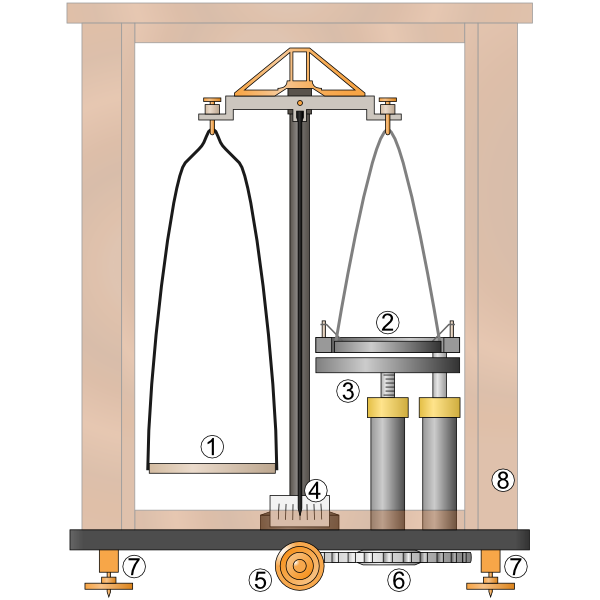
\includegraphics[scale=0.7]{PotWaageSchema.png}
	\caption{Schema der Potentialwaage: \small{\emph{1. Gewichtauflage; 2. obere Kondensatorplatte; 3. untere Kondensatorplatte; 4. Lot; 5. Arretierung; 6. Justierrad der unteren Kondensatorplatte; 7. Justierschrauben; 8. Holz-/Glas-Gehäuse}}\protect\footnotemark}
	\label{fig:PotWaageSchema}
\end{figure}
\footnotetext{Quelle: https://lp.uni-goettingen.de/get/text/3664, abgerufen am 06.09.2014}

Die Gewichte sollten nur mit einer Pinzette auf die Waage gelegt werden, da schon der kleinste Fettfleck ihre Masse beträchtlich ändern könnte und so die Messung verfälscht.
Außerdem muss bei Betrieb der Waage, also angelegter Hochspannung, aus Sicherheitsgründen das Fenster geschlossen sein.\\

\textbf{Messung 1:}
Zuerst wird die Waage arretiert, um 3g auf die Waagschale zu legen.
Dann wird eine Spannung $U$ (2, 3, 4, 5 kV) angelegt und die Arretierung gelöst.
Sollte die Waage kippen, muss der Plattenabstand $d$ des Kondensators verkleinert werden.
Anschließend wird der Plattenabstand vergrößert, bis die obere Kondensatorplatte abgehoben wird.
Diesen Wert notiert man dann.
All dies wird noch für eine aufgelegte Masse von $m=4$g wiederholt.\\  
\textbf{Messung 2:}
Nun wird der Plattenabstand auf $d=2, 2.5, 3, 4\,$mm fest eingestellt.
Für mindestens 3 verschiedene Massen $1\,\text{g}\leq m \leq 4\,\text{g}$ wird durch Vermindern der angelegten Spannung $U$ die Spannung bestimmt, bei der die Waage kippt.

\section{Auswertung}
\label{sec:auswertung}
Bevor mit der eigentlichen Auswertung begonnen wird, berechnen wir die effektive Fläche $A$ des Kondensators, da hier die kapazitiven Effekte zwischen Ring und Platte beachtet werden müssen.
Diese berechnet man nach der Formel aus dem Praktikumshandbuch:
\begin{align*}
 A=\pi (r^2+ra)
\end{align*}
Dabei ist $r=40\,$mm der Radius der oberen Platte ohne Schutzring und $a=1\,$mm die Breite des Schlitzes.
So ergibt sich: $$A=5.152 \cdot 10^{-3}\,\si{\meter^2}$$
Im folgenden wird mit einer Erdbeschleunigung von $g=9.81\,\si{\meter\per\second^2}$ gerechnet.

\subsection{konstante Kraft}
Aus Gleichung \eqref{eq:PotWaage} folgt eine lineare Abhängigkeit zwischen der Spannung $U$ und dem Plattenabstand $d$ für eine konstante Gewichtskraft, also wenn die Masse $m$ fest ist.
\begin{align}
 d= \sqrt{\frac{\varepsilon_0 A}{2mg}} \cdot U
\end{align}
In der nachfolgenden Abbildung \ref{fig:d(U)} ist diese Abhängigkeit dargestellt.
\begin{figure}[!htb]
 \centering
 % GNUPLOT: LaTeX picture with Postscript
\begingroup
  \makeatletter
  \providecommand\color[2][]{%
    \GenericError{(gnuplot) \space\space\space\@spaces}{%
      Package color not loaded in conjunction with
      terminal option `colourtext'%
    }{See the gnuplot documentation for explanation.%
    }{Either use 'blacktext' in gnuplot or load the package
      color.sty in LaTeX.}%
    \renewcommand\color[2][]{}%
  }%
  \providecommand\includegraphics[2][]{%
    \GenericError{(gnuplot) \space\space\space\@spaces}{%
      Package graphicx or graphics not loaded%
    }{See the gnuplot documentation for explanation.%
    }{The gnuplot epslatex terminal needs graphicx.sty or graphics.sty.}%
    \renewcommand\includegraphics[2][]{}%
  }%
  \providecommand\rotatebox[2]{#2}%
  \@ifundefined{ifGPcolor}{%
    \newif\ifGPcolor
    \GPcolortrue
  }{}%
  \@ifundefined{ifGPblacktext}{%
    \newif\ifGPblacktext
    \GPblacktexttrue
  }{}%
  % define a \g@addto@macro without @ in the name:
  \let\gplgaddtomacro\g@addto@macro
  % define empty templates for all commands taking text:
  \gdef\gplbacktext{}%
  \gdef\gplfronttext{}%
  \makeatother
  \ifGPblacktext
    % no textcolor at all
    \def\colorrgb#1{}%
    \def\colorgray#1{}%
  \else
    % gray or color?
    \ifGPcolor
      \def\colorrgb#1{\color[rgb]{#1}}%
      \def\colorgray#1{\color[gray]{#1}}%
      \expandafter\def\csname LTw\endcsname{\color{white}}%
      \expandafter\def\csname LTb\endcsname{\color{black}}%
      \expandafter\def\csname LTa\endcsname{\color{black}}%
      \expandafter\def\csname LT0\endcsname{\color[rgb]{1,0,0}}%
      \expandafter\def\csname LT1\endcsname{\color[rgb]{0,1,0}}%
      \expandafter\def\csname LT2\endcsname{\color[rgb]{0,0,1}}%
      \expandafter\def\csname LT3\endcsname{\color[rgb]{1,0,1}}%
      \expandafter\def\csname LT4\endcsname{\color[rgb]{0,1,1}}%
      \expandafter\def\csname LT5\endcsname{\color[rgb]{1,1,0}}%
      \expandafter\def\csname LT6\endcsname{\color[rgb]{0,0,0}}%
      \expandafter\def\csname LT7\endcsname{\color[rgb]{1,0.3,0}}%
      \expandafter\def\csname LT8\endcsname{\color[rgb]{0.5,0.5,0.5}}%
    \else
      % gray
      \def\colorrgb#1{\color{black}}%
      \def\colorgray#1{\color[gray]{#1}}%
      \expandafter\def\csname LTw\endcsname{\color{white}}%
      \expandafter\def\csname LTb\endcsname{\color{black}}%
      \expandafter\def\csname LTa\endcsname{\color{black}}%
      \expandafter\def\csname LT0\endcsname{\color{black}}%
      \expandafter\def\csname LT1\endcsname{\color{black}}%
      \expandafter\def\csname LT2\endcsname{\color{black}}%
      \expandafter\def\csname LT3\endcsname{\color{black}}%
      \expandafter\def\csname LT4\endcsname{\color{black}}%
      \expandafter\def\csname LT5\endcsname{\color{black}}%
      \expandafter\def\csname LT6\endcsname{\color{black}}%
      \expandafter\def\csname LT7\endcsname{\color{black}}%
      \expandafter\def\csname LT8\endcsname{\color{black}}%
    \fi
  \fi
  \setlength{\unitlength}{0.0500bp}%
  \begin{picture}(7200.00,5040.00)%
    \gplgaddtomacro\gplbacktext{%
      \csname LTb\endcsname%
      \put(946,704){\makebox(0,0)[r]{\strut{}-1}}%
      \put(946,1111){\makebox(0,0)[r]{\strut{}-0.5}}%
      \put(946,1518){\makebox(0,0)[r]{\strut{} 0}}%
      \put(946,1925){\makebox(0,0)[r]{\strut{} 0.5}}%
      \put(946,2332){\makebox(0,0)[r]{\strut{} 1}}%
      \put(946,2740){\makebox(0,0)[r]{\strut{} 1.5}}%
      \put(946,3147){\makebox(0,0)[r]{\strut{} 2}}%
      \put(946,3554){\makebox(0,0)[r]{\strut{} 2.5}}%
      \put(946,3961){\makebox(0,0)[r]{\strut{} 3}}%
      \put(946,4368){\makebox(0,0)[r]{\strut{} 3.5}}%
      \put(946,4775){\makebox(0,0)[r]{\strut{} 4}}%
      \put(1078,484){\makebox(0,0){\strut{} 0}}%
      \put(2032,484){\makebox(0,0){\strut{} 1}}%
      \put(2986,484){\makebox(0,0){\strut{} 2}}%
      \put(3941,484){\makebox(0,0){\strut{} 3}}%
      \put(4895,484){\makebox(0,0){\strut{} 4}}%
      \put(5849,484){\makebox(0,0){\strut{} 5}}%
      \put(6803,484){\makebox(0,0){\strut{} 6}}%
      \put(176,2739){\rotatebox{-270}{\makebox(0,0){\strut{}Plattenabstand [mm]}}}%
      \put(3940,154){\makebox(0,0){\strut{}Spannung [kV]}}%
    }%
    \gplgaddtomacro\gplfronttext{%
      \csname LTb\endcsname%
      \put(3322,4602){\makebox(0,0)[r]{\strut{}Messwerte $m=3\,$g}}%
      \csname LTb\endcsname%
      \put(3322,4382){\makebox(0,0)[r]{\strut{}Fit für $m=3\,$g}}%
      \csname LTb\endcsname%
      \put(3322,4162){\makebox(0,0)[r]{\strut{}Messwerte $m=4\,$g}}%
      \csname LTb\endcsname%
      \put(3322,3942){\makebox(0,0)[r]{\strut{}Fit für $m=4\,$g}}%
    }%
    \gplbacktext
    \put(0,0){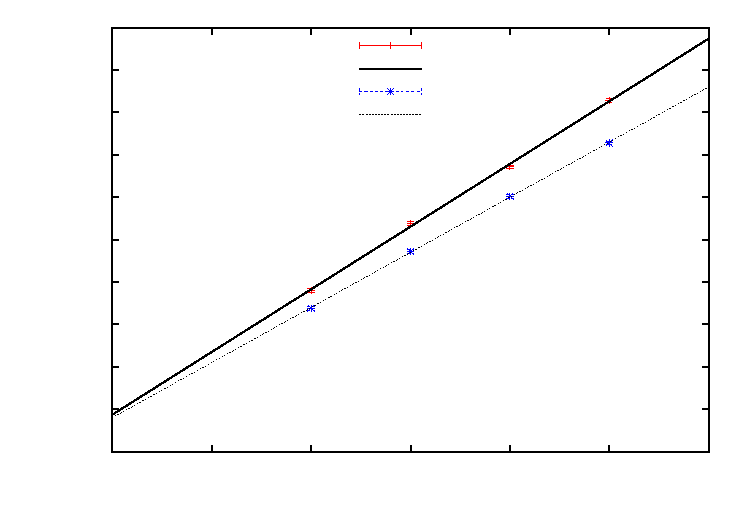
\includegraphics{messung1}}%
    \gplfronttext
  \end{picture}%
\endgroup

 \caption{Plattenabstand in Abängigkeit der angelegten Spannung}
 \label{fig:d(U)}
\end{figure}
Aus der Geradensteigung $k$ lässt sich durch Umstellen der obigen Formel $\varepsilon_0$ berechnen:
\begin{align*}
 \varepsilon_0=\frac{2mg}{A}\cdot k^2
\end{align*}

Es ergeben sich diese Steigungen $k$ und die daraus resultierenden Werte für $\varepsilon_0$:
\begin{table}[!htb]
 \centering
 \begin{tabular}{|c|c|c|}
  \hline
  \rule{0pt}{15pt}$m~[\si{\gram}]$&  $k~\left[\si[per-mode=fraction]{\milli\meter\per\kilo\volt}\right]$ & $\varepsilon_0~\left[10^{-12}\,\si[per-mode=fraction]{\ampere\second\per\volt\per\meter}\right]$\\
  \hline
  $3$ & $0.739\pm 0.017$ & $6.24 \pm 0.29$\\
  $4$ & $0.650\pm 0.007$ & $6.44 \pm 0.14$\\
  \hline
 \end{tabular}
 \caption{Geradensteigung und daraus berechnete elektrische Feldkonstante}
 \label{tab:messung1_k_epsilon0}
\end{table}

Es ergibt sich ein gewichteter Mittelwert von
\begin{empheq}[box=\shadowbox*]{align*}
  \overline{\varepsilon_0}=(6.40 \pm 0.13)\cdot 10^{-12}\,\si[per-mode=fraction]{\ampere\second\per\volt\per\meter}
\end{empheq}

Aus der linearen Regression folgt der Offset des Plattenabstandes als das Negative des y-Achsenabschnittes:\\
\begin{table}[!htb]
 \centering
 \begin{tabular}{|c|c|}
  \hline
  \rule{0pt}{15pt}$m~[\si{\gram}]$&  $\Delta ~ [\si{\milli\meter}]$\\
  \hline
  $3$ & $0.56 \pm 0.06$\\
  $4$ & $0.650\pm 0.007$\\
  \hline
 \end{tabular}
 \caption{Offset des Abstandes}
 \label{tab:messung1_Delta}
\end{table}

Es ergibt sich ein gewichteter Mittelwert von
\begin{empheq}[box=\shadowbox*]{align*}
  \overline{\Delta}=(0.595 \pm 0.022)\,\si{\milli\meter}
\end{empheq}
Für den wahren Plattenabstand $d_w$ muss also zum gemessenen Wert $d$ noch $\Delta$ addiert werden.

\subsection{konstanter Plattenabstand}
\begin{figure}[!htb]
 \centering
 % GNUPLOT: LaTeX picture with Postscript
\begingroup
  \makeatletter
  \providecommand\color[2][]{%
    \GenericError{(gnuplot) \space\space\space\@spaces}{%
      Package color not loaded in conjunction with
      terminal option `colourtext'%
    }{See the gnuplot documentation for explanation.%
    }{Either use 'blacktext' in gnuplot or load the package
      color.sty in LaTeX.}%
    \renewcommand\color[2][]{}%
  }%
  \providecommand\includegraphics[2][]{%
    \GenericError{(gnuplot) \space\space\space\@spaces}{%
      Package graphicx or graphics not loaded%
    }{See the gnuplot documentation for explanation.%
    }{The gnuplot epslatex terminal needs graphicx.sty or graphics.sty.}%
    \renewcommand\includegraphics[2][]{}%
  }%
  \providecommand\rotatebox[2]{#2}%
  \@ifundefined{ifGPcolor}{%
    \newif\ifGPcolor
    \GPcolortrue
  }{}%
  \@ifundefined{ifGPblacktext}{%
    \newif\ifGPblacktext
    \GPblacktexttrue
  }{}%
  % define a \g@addto@macro without @ in the name:
  \let\gplgaddtomacro\g@addto@macro
  % define empty templates for all commands taking text:
  \gdef\gplbacktext{}%
  \gdef\gplfronttext{}%
  \makeatother
  \ifGPblacktext
    % no textcolor at all
    \def\colorrgb#1{}%
    \def\colorgray#1{}%
  \else
    % gray or color?
    \ifGPcolor
      \def\colorrgb#1{\color[rgb]{#1}}%
      \def\colorgray#1{\color[gray]{#1}}%
      \expandafter\def\csname LTw\endcsname{\color{white}}%
      \expandafter\def\csname LTb\endcsname{\color{black}}%
      \expandafter\def\csname LTa\endcsname{\color{black}}%
      \expandafter\def\csname LT0\endcsname{\color[rgb]{1,0,0}}%
      \expandafter\def\csname LT1\endcsname{\color[rgb]{0,1,0}}%
      \expandafter\def\csname LT2\endcsname{\color[rgb]{0,0,1}}%
      \expandafter\def\csname LT3\endcsname{\color[rgb]{1,0,1}}%
      \expandafter\def\csname LT4\endcsname{\color[rgb]{0,1,1}}%
      \expandafter\def\csname LT5\endcsname{\color[rgb]{1,1,0}}%
      \expandafter\def\csname LT6\endcsname{\color[rgb]{0,0,0}}%
      \expandafter\def\csname LT7\endcsname{\color[rgb]{1,0.3,0}}%
      \expandafter\def\csname LT8\endcsname{\color[rgb]{0.5,0.5,0.5}}%
    \else
      % gray
      \def\colorrgb#1{\color{black}}%
      \def\colorgray#1{\color[gray]{#1}}%
      \expandafter\def\csname LTw\endcsname{\color{white}}%
      \expandafter\def\csname LTb\endcsname{\color{black}}%
      \expandafter\def\csname LTa\endcsname{\color{black}}%
      \expandafter\def\csname LT0\endcsname{\color{black}}%
      \expandafter\def\csname LT1\endcsname{\color{black}}%
      \expandafter\def\csname LT2\endcsname{\color{black}}%
      \expandafter\def\csname LT3\endcsname{\color{black}}%
      \expandafter\def\csname LT4\endcsname{\color{black}}%
      \expandafter\def\csname LT5\endcsname{\color{black}}%
      \expandafter\def\csname LT6\endcsname{\color{black}}%
      \expandafter\def\csname LT7\endcsname{\color{black}}%
      \expandafter\def\csname LT8\endcsname{\color{black}}%
    \fi
  \fi
  \setlength{\unitlength}{0.0500bp}%
  \begin{picture}(7200.00,5040.00)%
    \gplgaddtomacro\gplbacktext{%
      \csname LTb\endcsname%
      \put(1078,704){\makebox(0,0)[r]{\strut{} 0}}%
      \put(1078,1383){\makebox(0,0)[r]{\strut{} 0.01}}%
      \put(1078,2061){\makebox(0,0)[r]{\strut{} 0.02}}%
      \put(1078,2740){\makebox(0,0)[r]{\strut{} 0.03}}%
      \put(1078,3418){\makebox(0,0)[r]{\strut{} 0.04}}%
      \put(1078,4097){\makebox(0,0)[r]{\strut{} 0.05}}%
      \put(1078,4775){\makebox(0,0)[r]{\strut{} 0.06}}%
      \put(1210,484){\makebox(0,0){\strut{} 0}}%
      \put(2329,484){\makebox(0,0){\strut{} 5}}%
      \put(3447,484){\makebox(0,0){\strut{} 10}}%
      \put(4566,484){\makebox(0,0){\strut{} 15}}%
      \put(5684,484){\makebox(0,0){\strut{} 20}}%
      \put(6803,484){\makebox(0,0){\strut{} 25}}%
      \put(176,2739){\rotatebox{-270}{\makebox(0,0){\strut{}$F$ [N]}}}%
      \put(4006,154){\makebox(0,0){\strut{}$U^2$ [(kV)$^2$]}}%
    }%
    \gplgaddtomacro\gplfronttext{%
      \csname LTb\endcsname%
      \put(3850,4602){\makebox(0,0)[r]{\strut{}Messwerte $d=2\,$mm}}%
      \csname LTb\endcsname%
      \put(3850,4382){\makebox(0,0)[r]{\strut{}Fit für $d=2\,$mm}}%
      \csname LTb\endcsname%
      \put(3850,4162){\makebox(0,0)[r]{\strut{}Messwerte $d=2.5\,$mm}}%
      \csname LTb\endcsname%
      \put(3850,3942){\makebox(0,0)[r]{\strut{}Fit für $d=2.5\,$mm}}%
      \csname LTb\endcsname%
      \put(3850,3722){\makebox(0,0)[r]{\strut{}Messwerte $d=3\,$mm}}%
      \csname LTb\endcsname%
      \put(3850,3502){\makebox(0,0)[r]{\strut{}Fit für $d=3\,$mm}}%
      \csname LTb\endcsname%
      \put(3850,3282){\makebox(0,0)[r]{\strut{}Messwerte $d=4\,$mm}}%
      \csname LTb\endcsname%
      \put(3850,3062){\makebox(0,0)[r]{\strut{}Fit für $d=4\,$mm}}%
    }%
    \gplbacktext
    \put(0,0){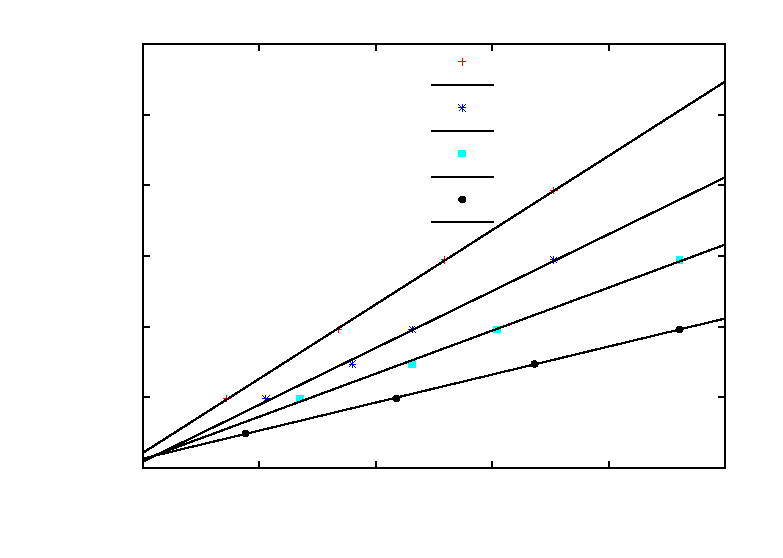
\includegraphics{messung2}}%
    \gplfronttext
  \end{picture}%
\endgroup

 \caption{Kraft in Abängigkeit des Quadrats der angelegten Spannung}
 \label{fig:F(U^2)}
\end{figure}

\begin{align}
 \varepsilon_0 &= k\cdot \frac{2d_w^2}{A}\\
 \sigma_{\varepsilon_0} &= \sqrt{\sigma_k^2\cdot\left(\frac{2d_w^2}{A}\right)^2+\sigma_{d_w}^2\cdot\left(\frac{4d_wk}{A}\right)^2}
\end{align}


\begin{table}[!htb]
	\centering
	\begin{tabular}{|c|c|c|c|}
		\hline
		\rule{0pt}{15pt}$d~[\si{\milli\meter}]$ &  $d_w ~ [\si{\milli\meter}]$ & $k$ [N/(kV)$^2$] & $\varepsilon_0 ~ \left[10^{-12}\,\si[per-mode=fraction]{\ampere\second\per\volt\per\meter}\right]$\\
		\hline
		$2.000 \pm 0.010$ & $2.595 \pm 0.024$ & $0.00226 \pm 0.00005$ & $5.92 \pm 0.16$ \\
$2.500 \pm 0.010$ & $3.095 \pm 0.024$ & $0.001680 \pm 0.000026$ & $6.25 \pm 0.14$ \\
$3.000 \pm 0.010$ & $3.595 \pm 0.024$ & $0.001288 \pm 0.000022$ & $6.46 \pm 0.14$ \\
$4.000 \pm 0.010$ & $4.595 \pm 0.024$ & $0.000870 \pm 0.000022$ & $7.13 \pm 0.20$ \\
		\hline
	\end{tabular}
	\caption{Werte dieser Messung}
	\label{tab:messung2}
\end{table}

Für $\varepsilon_0$ ergibt sich ein gewichteter Mittelwert von
\begin{empheq}[box=\shadowbox*]{align*}
  \overline{\varepsilon_0}=(6.37 \pm 0.08)\cdot 10^{-12}\,\si[per-mode=fraction]{\ampere\second\per\volt\per\meter}
\end{empheq}


\section{Diskussion}
\label{sec:diskussion}
Vergleicht man beide Werte für $\varepsilon_0$ untereinander, fällt auf, dass sie weniger als $1\%$ voneinander abweichen und der eine Wert im Fehlerintervall des jeweils anderen liegt.
Verglichen mit dem Literaturwert $\varepsilon_0\approx 8.854\cdot 10^{-12}\,\si[per-mode=fraction]{\ampere\second\per\volt\per\meter}$ ergibt sich jedoch eine erhebliche Abweichung von mehr als $25\%$.
Dies deutet also auf einen systematischen Fehler im Versuchsaufbau hin.


Die Annahme $\varepsilon_r=1$ kann auch weiter verwendet werden, da für alle anderen Medien als Vakuum $\varepsilon_r$ größer ist und so der gemessene Wert für $\varepsilon_0$ größer sein müsste.

\section{Anhang}

\end{document}
